\documentclass{listhesis}
% --- Listhesis builds on KOMA script report (scrreprt).
%     Class arguments are passed to that class.

% --- Add additional packages here using \usepackage{package-name}.

% --- Provide your thesis details here.
\setup{%
  % de,                   % uncomment if your thesis is in German
  author=Muhammad Sabir Amin, % your name
  title={Hardware in the Loop test bench designing for      \\     Embedded Controller used in food technology},
  date={December 15, 2019}, % submission date (today is used if unset)
  type=master,        % thesis type [master, bachelor, research, internship, diplom]
  advisor=Prof. Dr. Thomas Schumann, % your advisor (typically some PhD. student)
  supervisor=Prof. Dr. Herbert Krauß, % your supervisor
  % % uncomment the next lines if your thesis was carried out in industry
  company=PreciBake GmbH,
  externalAdvisor=Christian Höfer
}

\begin{document}
\maketitle
\cleardoublepage






\confirmation

% --- Thesis abstract.
%     For German thesis also provide an English version via the optional
%     argument: \anstract[English]{German}
\abstract{
Introduction of industry 4.0 have revolutionized the technology era by replacing manual systems. Every field of life is being automated for making processes fast, easy, reliable and efficient. Automated baking is being introduced on a commercial scale as it is more error prone and assures the food quality in bulk. Especially for bread and other bakery items the products are quite sensitive as the taste, quality, texture and color of the products are important to the customer and are critical for running a successful business. Different markets and restaurants are using technology based systems to maintain their standards and to meet a large customer requirement. Hence, more and more businesses wants to automate their systems. We need a fully running system which compromises of sensors, cameras and a processing unit and software which runs on top of the processing unit. Testing needs to be done in order to ensure that the system is running as expected and is error prone. Different test techniques are used on hardware and software. In this thesis, I have created a simulation system for such an automated baking platform which simulates the motors inside the food processing machine inorder to ensure that the commands issued by the processor are executed according to the input data. 

 



}
\makeabstract
\clearpage

% --- Content tables.
\
\tableofcontents
\clearpage
\listoffigures
\clearpage
\listoftables
\clearpage


% --- Your thesis starts here.
%     Use \chapter{}, \section{}, \subsection{}, \subsubsection{},
%     and \paragraph{} to structure your thesis.

\chapter{Introduction}
The implementation of innovation in the technology have increased in all areas of life and the food industry is one of the areas to be a part of industry 4.0. Increase in the number of products and baked items consumers is quite significant and this number requires systems to be automated and to be efficient. Bread and bakery products are one of the most popular consumer's purchased items and an example is that Germany consumes about 5.2 million tonnes of bread and bakery products per year. In case of the products from food industry the efficiency is not the only criteria of acceptance, the quality(taste and color) are quite an importance for customer satisfaction. This already large and increasing market requires automation focused on efficiency and quality.


\section{Project Objectives}
The purpose of the thesis is to design a hardware-in-the-loop test bench for embedded system used in food processing machines. This embedded controller will be used to control the next generation of dough sheeters made by Rondo Burgdorf AG~\cite{rondo}. This embedded system will be provided by PreciBake GmbH, it consists of an ARM-based embedded board and a 10.1” touch monitor in a joint housing. In the initial phase of the project the test basic features of the embedded controller and later on extensive testing will be done so that the functionality of the system and upcoming features is tested more efficiently by increasing the pace of testing and also improving the test coverage for better quality assurance. 
 \\

\section{Company Overview}
PreciBake® ~\cite{precibake} is an AI and sensor technology company providing software and hardware solutions to the food and beverage processing industry. The company was founded in 2012 in New York City by Laura Horstmann and Dr.-Ing. Ingo Stork-Wersborg with the initial goal to create AI applications for bakeries. Offices in Munich and Mumbai were founded in 2013 and 2014, respectively, to be able to serve the European and Asian markets. In 2018, the new brand PreciTaste®~\cite{precitaste} was introduced to acknowledge the extended customer base which currently includes equipment manufacturers as well as professional end users. Today, the company employs over 50 people worldwide. 

The company is working on multiple projects in the food and beverage processing industry like adding smart features (Virtual Baker, Virtual Quality Officer) to machinery, and also providing hardware and software development services. The main products of PreciBake® are: \\

\subsection{Virtual Baker™/AI agent}
The Virtual Baker (AI agent) is an add-on for ovens that lets customers automate oven controls and bake products according to their needs. Using Artificial Intelligence, the system recognizes
which baking goods are fed into the oven and in which quantities, selects the right baking program, and can react to differences in processes. The Virtual Baker learns the customer’s
desired baking process and then assists to ensure individual quality standards and easy oven operation.

\subsection{Virtual Quality Officer™}
The Virtual Quality Officer is an intelligent process monitoring and automation system for industrial customers that monitors baking lines with respect to relevant parameters such as size,
shape, consistency, or color of baked goods. If an error occurs, the system alerts the user, thus preventing wastage and minimizing costs. In addition, the assistance system can also be used
with fermentation processes, conveyor belts, and robots.

\subsection{BakeIT Cloud™/TasteOS}
The innovative web-based cloud system connects different bakery machinery together regardless of the manufacturer. This makes it possible to monitor and analyze all the baking processes at different locations. Moreover, the BakeIT Cloud enables communication between machines thus simplifying processes while also continuously optimizing them at the same time.
\newpage
\section{Fundamentals}

PreciBake is working on different food processing machines. Adding smart features to commercial ovens and providing controllers to dough processing machines are some of the company tasks. 
A brief overview of the equipment needed for the specific project are given below:

\subsection{Dough Sheeter}

A dough sheeter is a machine that rolls out pieces of dough to a desired thickness depending on the target product requirements which are then used to make different bakery products for commercial purposes. The resulting sheets are smooth, uniform and completed in a few minutes, a much shorter turnaround than rolling by hand. RONDO~\cite{rondo} is one of the leading companies in the area of developing and producing high quality machines and systems for the production of pastry of all types.  Given below in figure \ref{fig:rondosheeter}  show  the dough sheeter (a current model) having a basic controller and the figure \ref{fig:endproduct} is dough made with different number of layers based on the requirements.

\begin{figure}[!b]
  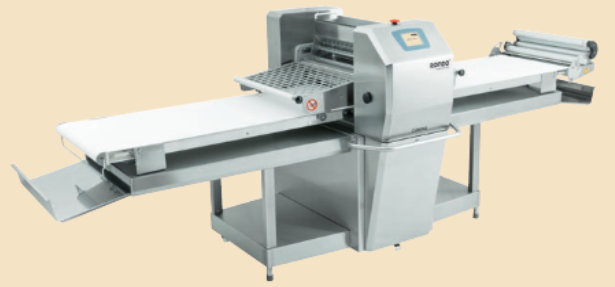
\includegraphics[width=0.7\linewidth]{rondosheeter.png}
  \centering
  \caption{Rondo Sheeter}
  \label{fig:rondosheeter}

  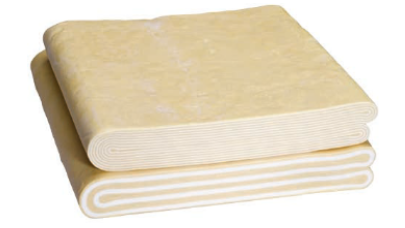
\includegraphics[width=0.5\linewidth]{endproduct.png}
  \centering
  \caption{End Product}
  \label{fig:endproduct}
\end{figure}





\subsection{Embedded Controller}
Rondo sheeter have an embedded controller for handling the different features of the dough sheeter. Precibake will be providing the support to RONDO in designing the hardware and software of this controller. The controller in figure \ref{fig:embeddedcontroller} consists of a ARM-based~\cite{arm} embedded board and a 10.1” touch monitor in a joint housing . The current models have an old controller with some basic features and old interface provided to RONDO by another company. For the upcoming models Precibake will be providing the Embedded controller to RONDO with better features and interface. 
\begin{figure}[h!]
  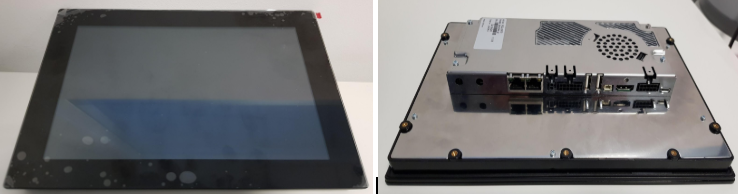
\includegraphics[width=\linewidth]{embeddedcontroller.png}
  \centering
  \caption{Embedded Controller from PreciBake}
  \label{fig:embeddedcontroller}
\end{figure}

\subsubsection{Features of the Embedded Controller}
Embedded controller have different features and ability to control the RONDO sheeter. Give below is a brief overview of the features and different interfaces of the RONDO controller. 

Connectivity Check:
Motors functionality check:
Default Recipies:
Custom Recipies:



\section{Outline}

In this section a brief overview of the steps included in the implementation of the project is given. 
\begin{itemize}


\item{Requirements Analysis }

After the market / literature overview decision will be made about the target approach and then target specific requirements will be analyzed.

\item{Designing and Implementation of Test Bench }

After understanding of the requirements and making decision the simulation will be implemented for making the test bench.

\item{Integration of project software and hardware}

After completion of the simulation the interfacing of the controller with the simulated RONDO sheeter will be implemented. 

\item{Performance Evaluation}

After interfacing the controller with the RONDO sheeter initial tests will be conducted to validate the performance of the test system. 

\item{Designing and Execution of Test Cases}

Performance evaluation will give an idea about the effectiveness and efficiency of the designed system and further extensive test cases will be designed.

\item{Results Analysis}

To verify the effectiveness of the test systems different test cases will be designed and run and the results will be analyzed and compared to the previous results(manual tests).

\end{itemize}






\chapter{Technical background}
\section{Hardware in the Loop} Hardware in the Loop (HiL) ~\cite{hil} simulation is a technique for performing system level testing of embedded systems in a comprehensive, cost-effective and repeatable manner. A real time simulation is required to interact with the under test system (Embedded controller). Figure \ref{fig:hil} shows an overview of the HiL system. 
\begin{figure}[h!]


  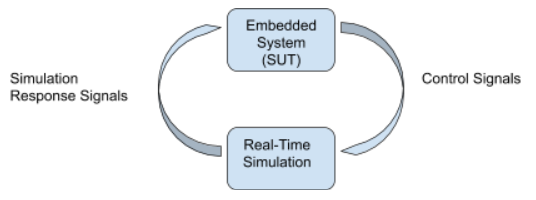
\includegraphics[width=0.7\linewidth]{hil.png}
  \centering
  \caption{Hardware in the Loop system (HiL)}
  \label{fig:hil}
\end{figure}
\par

\textbf{Hardware (Embedded System)}: Rondo sheeter have an embedded controller for handling the different features of the dough sheeter. Precibake will be providing the support to RONDO in designing the hardware and software of this controller. The controller (Figure 3.3) consists of a ARM-based embedded board and a 10.1” touch monitor in a joint housing . The current models have an old controller with some basic features and old interface provided to RONDO by another company. For the upcoming models (by the end of this year), Precibake will be providing the Embedded controller to RONDO with better features and interface.
Embedded system is a controller with a dedicated function within a larger mechanical or electrical system, often with real-time computing constraints. SANTOKA x2 ~\cite{arm} is used in the project. Santoka X2 consists of a cortex A9 processor. \\
\par
\section{Simulation} Simulation in an approximate imitation of the operation of a process or a system that represents the operation of the actual system over time. Simulation requires the development of a model that represents the key characteristics or behavior of the system/process.
\\
\par
\textbf{Matlab}: Matlab is a high level programming language and interactive environment for numerical computation , visualization and programming. Matlab is used to implement algorithms, creation of user interfaces and most importantly interfacing with programs written in other languages. Data analysis, algorithm development and modelling are other applications of matlab. different uses are signal processing and communication, image processing and test management.\\

\par
\textbf{Simulink}: Simulink is a Matlab-based graphical programming environment for modelling, simulating and analyzing multi domain dynamical systems, Its primary interface is graphical block diagramming tool and a customizable set of block libraries. Some of the block libraries to be used in the project are TCPIP, Instrument control toolbox .
\\
\par
\textbf{C++}: C++ is a statically typed, compiled, general purpose, case-sensitive, free-form  progarmming language that supports procedural, object oriented and generic programming. C++ is regarded as middle level programming language and it comprises of combination of both high level and low level language features. 
\\
\par
\section{Communication} HiL requires an embedded system and a simulation of the system with which the embedded system is interacting. The interaction requires some communication protocol and medium for successfull transfer and reception of the messages.
\\
\par
\textbf{EtherCAT}: Ethercat is an Ethernet based fieldbus system invented by Beckhoff Automation and this protocol is suitable for hard and soft real time computing requirements in automation technology. Ethercat is developed to apply ethernet for automation applications requiring short data update time with low communication cost and reduced hardware cost.
In case of the Simulation ethercat can be replaced by ethernet protocol and TCP/IP Protocol can be used for the Client server communication. 
\\
\par
\textbf{TCPIP}: TCPIP or Transmission Control Protocol/Internet Protocol is a suite of communication protocols used to interconnect network devices on the internet. This protocol specifies how data is exchanged over the internet by providing end-to-end communications that identify how it should be broken into packets, addressed, transmitted, routed and received at the destination. TCP/IP requires little central management, and it is designed to make network reliable, with the ability to recover automatically from the failure of any device on the network. TCP defines how applications can create channels of communication across a network. It also manages how a message is assembled into smaller packets before they are then transmitted over the internet and reassembled in the right order at the destination address
IP defines how to address and route each packet to make sure it reaches the right destination. Rach gateway computer on the network check this IP address to determine where to forward the message. 
\\
\par
\textbf{Nanomsg}: Nanomsg is a socket library that provides several communication patterns. It aims to make the networking layer fast, scalable and easy to use. Nanomsg is alternative to ZeroMQ, developed in C. It works on a wide range of operating systems with no further dependencies. The communicaiton patterns are basic blocks for building distributed systems and they can be combined to create a vast array of distributed applications. The following scalability protocols are available:\\
\\
1- PAIR-simple one to one communication\\
2- BUS-simple many to many communication\\
3- REQREP- allows to build clusters of stateless services to process user requests\\
4- PUBSUB- aggregates messages from multiple sources and load balances them among many destinations.\\
\par
\textbf{Protobuf}: Protocol Buffers are Google’s language neutral, platform neutral , extensible mechanism for serializing structured data. It is a data serializing protocol. The data to be sent can be structured once and then special generated code can be used to easily write and read structured data to and from a variety of data streams and using a variety of languages.  The design goals for protocol buffers are focused on simplicity and performance. Protobufs are widely used at google for storing and interchanging all kinds of structure information. 
\\

\section{Problem statement}
PreciBake GmbH is using Embedded system to control the functionality of RONDO sheeter according to requirements. The controller has the capability to send/receive messages from and to the sheeter and RONDO sheeter responds to these messages resulting the changing bhaviour of the motors in the sheeter. Testing of the embedded controller is done by sending message to rondo sheeter and monitoring the behavior of the motors and the machine overall. In this project the rondo sheeter will be replaced by a simulation of the motors and the funcitonality of the embedded controller will be analyzed based on the message sent from the embedded controller and the response from the simulation.

\chapter{Concept}

Food industry is of significant importance in the world and specifically in Germany because of the consumption of bakery products and the variety of items being used on a daily basis. this area needs to be brought under the umbrella of evolving technology and the introduction of the concept of Industry 4.0. The main idea of the project is to use the concept of Hardware in the loop in a different discipline of equipment used in the food industry. Previously HiL testing has been used in different areas because of its efficiency and easy handling. For the same reason embedded controller used in food area will be tested.

 

\section{Related work}
An overview of the importance of technology in food industry and different projects where HiL hase been used is discussed below.

\subsection{Consumption of Bakery Products}
Bakery market retail value in the world is 338.7 billion dollars and and annual growth of 4.7 percent and Germany have a market share of 4.9 percent in it. Also Germany is on of the 10 top importers in the world for bakery products(reference will be added)
\\

\subsection{Electronic Control Unit Testing using HiL}
ECU(Electronic Control Unit) or Electronic Control Module is an embedded controller used in automotive electronics to control the electrical system or subsystem of a vehicle. ~\cite{ecuhil}In this task a car simulation is designed using different tools and the ECU is used to analyze the response before testing it in an actual vehicle The purpose of HIL testing is the great number f the possible system states, automated testing, greater cases coverage and complete reproducibility. A dSpace simulator is used for controlling the input/output and all the CAN signals of the ECU. \\

\subsection{HIL testing of Car Infotainment System}
Infotainment system is a combination of Information and entertainment providing software and hardware module designed for human interaction in the vehicles. Hardware in the loop testing is used to test the infotainment systems before installing the system in the cars. dSPACE simulator is used for the purpose of HIL simulation where the different input (entertainment) signals are captured from the multimedia system(CD player, DVD player and display) while other signals(information) signals are captured from Sensors, Relays, resistors and ECU unit. Audi A5 uses the simulator ~\cite{infotainment} to test the Infotainment system for their car models\\



\subsection{HiL based ADAs Testing}
Autonomous driving is connected to the capability of verification and validation of advanced driver assistance system and this is on of the main challenge. Security, reliability and acceptance of the self driving cars requires a lot of testing. Hardware in the loop testing methods offer a great advantage for the validation and verification of the system in an early development stage making the test system significant for automotive industry. Multiple input signals from sensors, radars and cameras are used in the HIL simulated plant model and unit under tests.



\section{Goals of Thesis}
The goal of this thesis is to design and implement a HiL test bench for the embedded controller and to anaylze the effeciency of the test bench. The following features to be implemented and given below are the objectives that will be attained during the project. \\
\\
1-	Designing and implementation of a simulation for the RONDO machine behavior \\
2-	Interfacing the simulation with the real embedded controller. \\
3-	Implementing of basic test cases for validity/verification of the system. \\
4-	Designing and implementing of extensive tests for performance verification and acceptance  \\
5-	Documentation \\
6-	Measuring different variables(Test time, accuracy) for Evaluation purpose. \\


\section{Approach}
The steps followed to develop the hardware in the loop test bench for embedded controller are as follows:
\begin{itemize}
  \item Understanding the Idea: In this step, the pirpose is to understand the concept of Hardware in the Loop and its applications for the purpose of implementation it in this specific project. 

  \item Literature Review: Find and read relevant work that has already been done in the area of testing and specifically in hardware in the loop testing. A method will be chosen where the matlab and simulink are interfaced to the board to acheive the purpose testing.

  \item Design: Here we decide which technologies to use and how to design our system for optimal results. Also, it will be decided how to analyze the result of the new implemented test bench and to compare it to the manual testing.

  \item Implementation: Implement of the test bench design will be done.
  \item Evaluation and Testing: Compare the performance of implemented test bench to the previously deployed (manual testing) system.
\end{itemize}





\section{Implementation of the actual setup Embedded Controller}
The Rondo Controller (GUI) has the code for all the functionalities of the machine. The project is implemented in C++ using Qt Creator. Embedded controller have the capability to verify basic functionality of the RONDO machine and also an extensive implementation of different recipe based on the user input and also on the requirements of RONDO for their customers. Some examples of the recipe from RONDO are croissants, rolls, etc. In the actual scenario the Embedded controller is working as a server and RONDO sheeter is working as a client.
Embedded controller is sending the SERVO control message based on which the rondo machine is working while in response the RONDO sheeter is sending just a STATUS message to confirm with a notification of YES NO or an error message. 




\subsection{Embedded Controller features and functionality}
Embedded controller is coded my PreciBake GmbH based on the RONDO requirements for their machines and according to the customer requirements. Different features  and functions that are a part of the Embedded controller  . (to be explained) 

\begin{figure}
  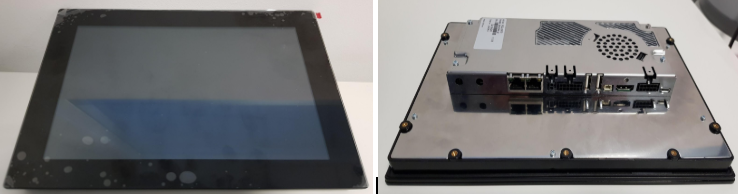
\includegraphics[width=\linewidth]{embeddedcontroller.png}
  \centering
  \caption{Embedded Controller from PreciBake}
  \label{fig:embeddedcontroller}
\end{figure}



\subsection{Rondo Sheeter features and functionality}
RONDO sheeter used in this project is COMPASS 4.0 version having 4 motors and servo drives that can be accessed and controlled over TCPIP. Given below are pictures and bried introduction of different parts of the RONDO Machine.

\begin{figure}
  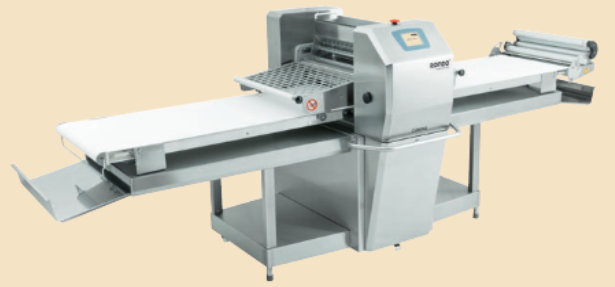
\includegraphics[width=0.7\linewidth]{rondosheeter.png}
  \centering
  \caption{Rondo Sheeter}
  \label{fig:rondosheeter}
\end{figure}



\newpage


\chapter{Project Implementation}
The controller have different functions and testing the controller means to start from the basic features. In the initial stage the controller is set to select the motor and assign a specific velocity to the motors. This is to verify the functionality of the board the board is connected to the RONDO machine and then the features are verified. THe controller creates the message that needs to be sent to the actual machine. This message is then encapsulated/structured in Protobuf buffer. Protobuf is a message structuring from google and used in industrial applications. After the message is structured in protobuf it is sent over EhterCAT/Ethernet using the Nanomsg protocol. In case of the simulation the message being structured in protof and sent over nanomsg needed to be retrieved at the simulation end. For this purpose the message is received in C++ and the message is decoded. FUnction to decode is onDataReceived() where the structure and destructuring is programmed. This message is then sent to matlab where the motor response simulation is run \ref{fig:implementation}.



\begin{figure}
  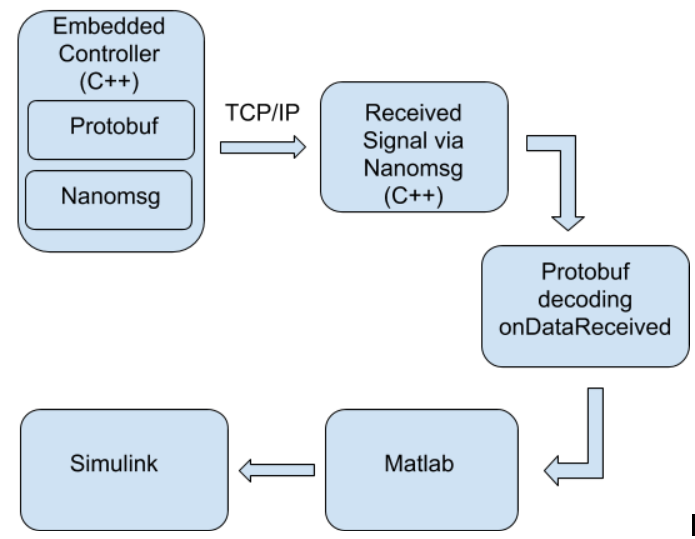
\includegraphics[width=0.7\linewidth]{implementation.png}
  \centering
  \caption{Implementation flow chart}
  \label{fig:implementation}
\end{figure}


\section{C++ Implementaiton (to be explained in detail}
The Rondo Controller (GUI) has the code for all the functionalities of the machine. The controller have different functions and testing the controller means to start from the basic features. In the initial stage the controller is set to select the motor and assign a specific velocity to the motors. This is to
verify the functionality of the board the board is connected to the RONDO machine and then the features are verified. The controller creates the message that needs to be sent to the actual machine. This message is then encapsulated/structured in Protobuf buffer. Protobuf is a message structuring from google and used in industrial applications. After the message is structured in protobuf it is sent over EhterCAT/Ethernet using the Nanomsg protocol. In case of the simulation the message being structured in protobuf and sent over nanomsg needed to be retrieved at the simulation end. For this purpose the message is received in C++ and the message is decoded. FUnction to decode is onDataReceived() where the structure and destructuring is programmed. This message is then sent to matlab where the motor response simulation is run.




\section{Matlab Implementation}
Matlab is used to code the behaviour of the rondo controller. Based on the input signal the motor is selected and a specific velocity is assigned to it and the veliocity can be seen on the scope. Matlab is used to get thhe input data from the lookup table. 
\section{Simulink}
\section{Communication between C++ and Matlab}


\chapter{Verificaiton and Validation}
In this chapter the the test bench designed is used to test the basic features of the embedded controller. The implementation of the project is discussed in the previous chapter and now the project funcitonality is being verified and test cases are designed for the verificaiton purpose. 

\section{Basic Testing}
As deiscused in section 1.---- the rondo controller have differnt deatures and interfaces based on the requirements. For example cconnectivity check.

\subsection{Connectivity Check}
The RONDO controller after being connected to the RONDO sheeter gives a notificiton of being online(not OFFLINE to be specific). To connect the shetter and controller, both the devices are needed to be on the same network and the RONDO controller works as a client and is looking for available devices with IP 0.0.0.0 and the IP address of the target machine needes to be assigned (example i given in the picture below). Server connects to the client via NANOMSG nnrecv. nnsend is connected to nnrecv and connection is established. thois connection verificaiton can be seen on the footer of the controller and the OFFLINE message is remove. Given below is a short test case to verify the connectivity.

\subsection{Motor Functionality Test}
RONDO controller is connected to the RONDO sheeter and the basic working of the motors can be verified as SMOKE test of the Sheeter. In this case the motor number can be selected and a specific velocity can be assigned to it and the response of the motor can be seen. In case of the simulation the motor number is assigned and in response the motor response can be seen on the screen in matlab. It is a running graph showing a specific velocity responding to input message. In this feature of the controller, individual motor can be selected and velocity can be assigned to it. A test case to verify this feature can be seen below. 


\section {Recipie Testing} 
RONDO CONTROLLER have the following recipies by default accoriding to the RONDO requriements. test cases are designed to verify the recepies.



\chapter{Conclusion and Outlook}

\section{Section}
\section{Future Work}

\newpage


% --- Bibliography
\cleardoublepage

%---------------------------------------------------------------------------------------------------------------

\medskip
\bibliographystyle{plain}
\begin{thebibliography}{100}



\bibitem{precibake} 
PreciBake GmbH,
\\\texttt{http://www.precibake.com} 

\bibitem{precitaste} 
PreciTaste,
\\\texttt{http://www.precitaste.com} 

\bibitem{rondo} 
Rondo Burgdorf AG,
\\\texttt{https://www.rondo-online.com/en} 

\bibitem{arm} Cortex A9, ``Technical Reference Manual," \emph{Revision: r4p1}, 2008 2012.


\bibitem{hil} Ledin, Jim A., ``Embedded Systems Programming," \emph{Hardware-in-the-Loop Simulation}, pp. 473-480, February 1999.


\bibitem{adatest}Feilhauer, M. and Haering, J. and Wyatt, S., Current Approaches in HiL-Based ADAS Testing \emph {SAE International Journal of Commercial Vehicles}, 63-69, 2016.

\bibitem{ecuhil} Daniel Lemp, Adam Opel AG,
Susanne Köhl, dSPACE GmbH,
Markus Plöger, dSPACE GmbH ., ``Steuergeräte-Verbundtests mittels
Hardware-in-the-Loop-Simulation," \emph{ECU Network Testing by HiL simulation}, ATZ10, 2003.

\bibitem{infotainment} ``Infotainment HIL Simulator at Audi", 2007.


\end{thebibliography}

%---------------------------------------------------------------------------------------------------------------






%\bibliography{thesis}

% --- Mandatory confirmation.
%\confirmation

\end{document}

%%% Local Variables:
%%% mode: latex
%%% TeX-master: t
%%% End:
